\documentclass[english]{beamer} %,handout
\usepackage{amsmath}
\usepackage{graphicx}
\usepackage[cjk,hangul,usecjkt1font]{kotex}

\makeatletter

\usepackage{listings}
\setbeamertemplate{footline}[frame number]
\setbeamercovered{transparent}

\usecolortheme{kesl}

\usepackage[absolute,overlay]{textpos}
\setlength{\TPHorizModule}{\paperwidth}
\setlength{\TPVertModule}{\paperheight}
\textblockorigin{0mm}{0mm}
 
\usepackage{babel}
\beamertemplatenavigationsymbolsempty
\usepackage{verbatim}
\begin{document}

\title[Memory Scalability]{
경량 로그 기반 지연 업데이트 기법을 활용한 리눅스 커널 확장성 향상 \\
\small{A Lightweight Log-based Deferred Update
for \\Linux Kernel Scalability}}

\author{Joohyun Kyong}
\institute[Kookmin University]
{
  School of Computer Science\\
  Kookmin University\\
  Thesis advisor: Sung-soo Lim
}

\setbeamercovered{dynamic} 
%TODO Audit Words, reduce

\begin{frame}
  \titlepage
\end{frame}

\begin{frame}{40 Years of Microprocessor Trend Data}
\pgfdeclareimage[width=\paperwidth]{cpu_1}{.//slides/cpu_1}
\begin{textblock}{1}(0,0)
\pgfuseimage<+->{cpu_1}
\end{textblock}
\end{frame}


\begin{frame}{40 Years of Microprocessor Trend Data}
\pgfdeclareimage[width=\paperwidth]{cpu_2}{.//slides/cpu_2}
\begin{textblock}{1}(0,0)
\pgfuseimage<+->{cpu_2}
\end{textblock}
\end{frame}

\begin{frame}{40 Years of Microprocessor Trend Data}
\pgfdeclareimage[width=\paperwidth]{cpu_3}{.//slides/cpu_3}
\begin{textblock}{1}(0,0)
\pgfuseimage<+->{cpu_3}
\end{textblock}
\end{frame}


\begin{frame}{40 Years of Microprocessor Trend Data}
\pgfdeclareimage[width=\paperwidth]{cpu_4}{.//slides/cpu_4}
\begin{textblock}{1}(0,0)
\pgfuseimage<+->{cpu_4}
\end{textblock}
\end{frame}

\begin{frame}{40 Years of Microprocessor Trend Data}
\pgfdeclareimage[width=\paperwidth]{cpu_5}{.//slides/cpu_5}
\begin{textblock}{1}(0,0)
\pgfuseimage<+->{cpu_5}
\end{textblock}
\end{frame}



\begin{frame}{OS Kernel Scalability Histroy}
\pgfdeclareimage[width=\paperwidth]{history}{.//slides/history}
\begin{textblock}{1}(0,0)
\pgfuseimage<+->{history}
\end{textblock}
\end{frame}



\begin{frame}{OS Kernel Scalability Histroy}
\pgfdeclareimage[width=\paperwidth]{history}{.//slides/history}
\begin{textblock}{1}(0,0)
\pgfuseimage<+->{history}
\end{textblock}
\end{frame}


\begin{frame}{OS Kernel Scalability Histroy}
\end{frame}


\begin{frame}{OS Kernel Scalability Histroy}
\end{frame}


\begin{frame}{OS Kernel Scalability Histroy}
\end{frame}


\begin{frame}{OS Kernel Scalability Histroy}
\end{frame}

\begin{frame}{Performance Scalability}
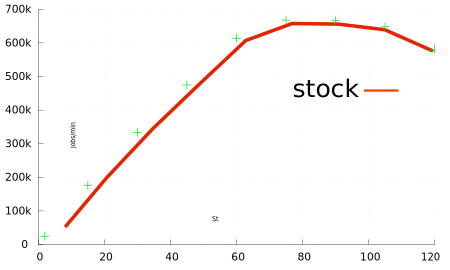
\includegraphics[scale=0.8]{graph/aim7_default}
\end{frame}

\begin{frame}{Performance Scalability}
\includegraphics[scale=0.8]{graph/aim7_default_2}
\end{frame}

\begin{frame}{Performance Scalability}
\includegraphics[scale=0.8]{graph/aim7_default_3}
\end{frame}

\begin{frame}{OS Kernel Scalability}
    \begin{itemize}[<+-| alert@+>]
    \item OS kernel scalability is an important part for the whole the system
    parallelism.
    \item If the kernel does not scale, applications will not scale.
    \end{itemize}
\end{frame}


\begin{frame}{Lock Profile on 120 core}
\includegraphics[scale=0.8]{graph/aim7_default_4}
\end{frame}


\begin{frame}{Wait time to acquire the lock}
\includegraphics[scale=0.8]{fig/lockstat}
\end{frame}

\begin{frame}{Wait time to acquire the lock}
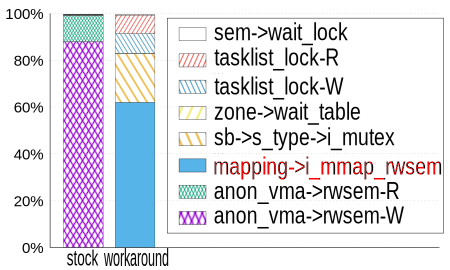
\includegraphics[scale=0.8]{fig/lockstat2}
\end{frame}


\begin{frame}{Update Serialization}
\pgfdeclareimage[width=\paperwidth]{update}{.//slides/update}
\begin{textblock}{1}(0,0)
\pgfuseimage<+->{update}
\end{textblock}
\end{frame}

\begin{frame}{High update rate Data Structuer}
\end{frame}

\begin{frame}{Update-heavy Data structure}
\end{frame}


\begin{frame}{Update-heavy Data structure}
\end{frame}

\begin{frame}{Non-blocking Data Structure}
\end{frame}


\begin{frame}{Non-blocking Data Structure}
\end{frame}


\begin{frame}{Non-blocking Data Structure}
\end{frame}


\begin{frame}{Non-blocking Data Structure}
\end{frame}


\begin{frame}{Cache communication bottlenect}
\end{frame}


\begin{frame}{Cache communication bottlenect}
\end{frame}


\begin{frame}{Cache communication bottlenect}
\end{frame}


\begin{frame}{Cache communication bottlenect}
\end{frame}

\begin{frame}{Cache communication bottlenect}
\end{frame}



\begin{frame}{Approach: Log-based Concurrent Update}
\end{frame}


\begin{frame}{Approach: Log-based Concurrent Update}
\end{frame}


\begin{frame}{Approach: Log-based Concurrent Update}
\end{frame}


\begin{frame}{Advantages of eliminating time-stamp counters}
\end{frame}


\begin{frame}{Contributions}
    \begin{itemize}[<+-| alert@+>]
	\item Removing time-stamp counters and eliminating the sources of limiting
	performance scalability in update-heavy data structures.
	\item  Applying the LDU in Linux kernel to two reverse mapping(anonymous, file)
	on an 120 core system to reduce fork scalability bottleneck.
	\item Our design improved throughput and execution time from 1.5x through 2.7x
	on 120 core.
	\end{itemize}
\end{frame}


\begin{frame}{Outline}
	\begin{itemize}
	\item Design
	\begin{itemize}
	\item Approach
	\item Example 
	\end{itemize}
	\item Applying the Linux kernel
	\item Implementation
	\item Evaluation
	\end{itemize}
\end{frame}


\begin{frame}{Design}
\end{frame}



\begin{frame}{Why the OpLog needs the time-stamp counter?}
A process logs an insert operation to the per-core memory, then
it migrates to another core, and it logs a remove operation, which must
eventually execute after the insert operation[OpLog].
\end{frame}



\begin{frame}{Log Example}
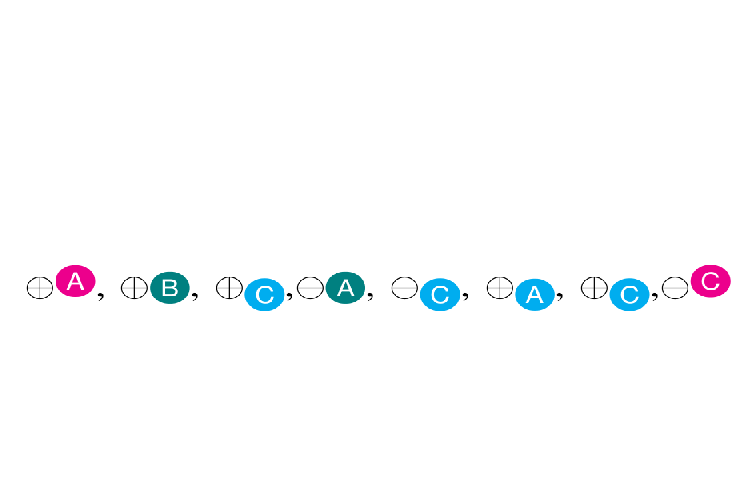
\includegraphics[scale=0.5]{fig/example_1}
\end{frame}


\begin{frame}{Cancelable - Log}
\includegraphics[scale=0.5]{fig/example_us}
\end{frame}


\begin{frame}{Update-side removing}
\includegraphics[scale=0.5]{fig/example_us}
\end{frame}

\begin{frame}{remain - Log}
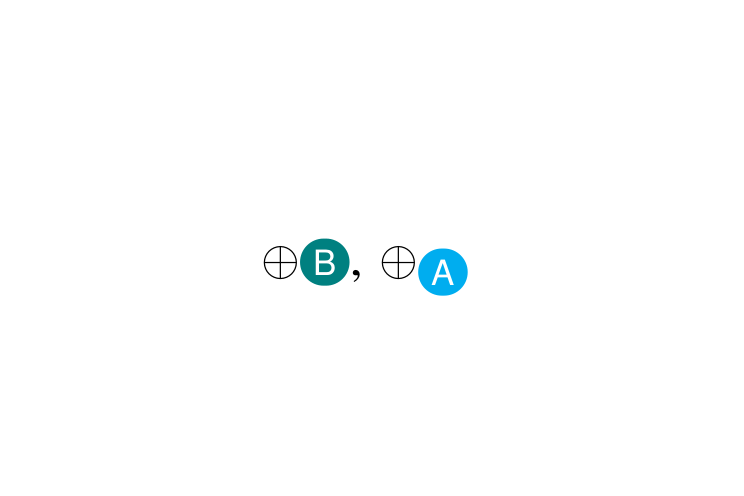
\includegraphics[scale=0.5]{fig/remain}
\end{frame}

\begin{frame}{Garbage logs}
\includegraphics[scale=0.5]{fig/example_gl}
\end{frame}

\begin{frame}{Reusing garbage}

\end{frame}


\begin{frame}{Additional approach}
	\begin{itemize}
	\item Periodically applies the operation logs.
	\begin{itemize}
	\item To reduce memory usage and to keep the log from growing without
	end.
	\item Similar with the method of previous OpLog’s batching
	updates and flat combining(FC)’s combiner thread.
	\end{itemize}
	\item Use non-blocking queue.
	\begin{itemize}
	  \item Regardless of the per-core queue or the global
	  queue.
	  \item Multiple producers and single consumer based non-blocking queue
	  thereby reducing the CAS operations.
	\end{itemize}
	\end{itemize}
\end{frame}


\begin{frame}{Example}
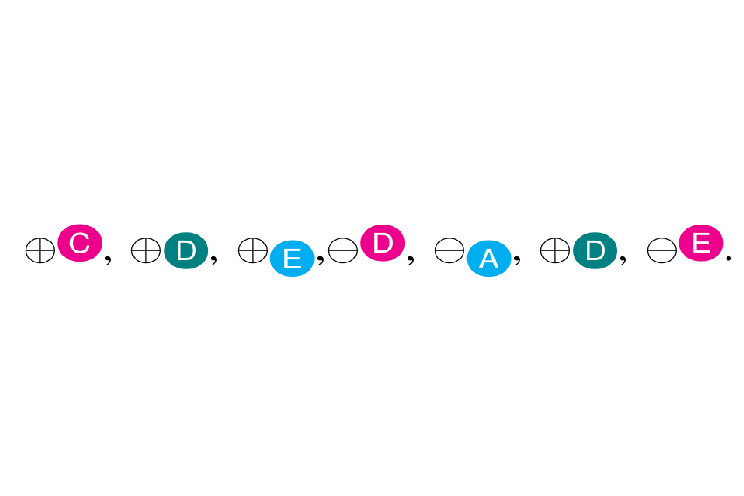
\includegraphics[scale=0.5]{fig/example}
\end{frame}


\begin{frame}{Example}
\pgfdeclareimage[width=\paperwidth]{ldu_1}{.//slides/ldu_1}
\begin{textblock}{1}(0,0)
\pgfuseimage<+->{ldu_1}
\end{textblock}
\end{frame}

\begin{frame}{Example}
\pgfdeclareimage[width=\paperwidth]{ldu_2}{.//slides/ldu_2}
\begin{textblock}{1}(0,0)
\pgfuseimage<+->{ldu_2}
\end{textblock}
\end{frame}

\begin{frame}{Example}
\pgfdeclareimage[width=\paperwidth]{ldu_3}{.//slides/ldu_3}
\begin{textblock}{1}(0,0)
\pgfuseimage<+->{ldu_3}
\end{textblock}
\end{frame}


\begin{frame}{Example}
\pgfdeclareimage[width=\paperwidth]{ldu_4}{.//slides/ldu_4}
\begin{textblock}{1}(0,0)
\pgfuseimage<+->{ldu_4}
\end{textblock}
\end{frame}


\begin{frame}{Example}
\pgfdeclareimage[width=\paperwidth]{ldu_5}{.//slides/ldu_5}
\begin{textblock}{1}(0,0)
\pgfuseimage<+->{ldu_5}
\end{textblock}
\end{frame}


\begin{frame}{Example}
\pgfdeclareimage[width=\paperwidth]{ldu_6}{.//slides/ldu_6}
\begin{textblock}{1}(0,0)
\pgfuseimage<+->{ldu_6}
\end{textblock}
\end{frame}


\begin{frame}{Example}
\pgfdeclareimage[width=\paperwidth]{ldu_7}{.//slides/ldu_7}
\begin{textblock}{1}(0,0)
\pgfuseimage<+->{ldu_7}
\end{textblock}
\end{frame}


\begin{frame}{Example}
\pgfdeclareimage[width=\paperwidth]{ldu_8}{.//slides/ldu_8}
\begin{textblock}{1}(0,0)
\pgfuseimage<+->{ldu_8}
\end{textblock}
\end{frame}


\begin{frame}{Example}
\pgfdeclareimage[width=\paperwidth]{ldu_9}{.//slides/ldu_9}
\begin{textblock}{1}(0,0)
\pgfuseimage<+->{ldu_9}
\end{textblock}
\end{frame}

\begin{frame}{Example}
\pgfdeclareimage[width=\paperwidth]{ldu_10}{.//slides/ldu_10}
\begin{textblock}{1}(0,0)
\pgfuseimage<+->{ldu_10}
\end{textblock}
\end{frame}


\begin{frame}{Applying the Linux kernel}
    \begin{itemize}[<+-| alert@+>]
    \item The Linux reverse page mapping(rmap).
    \item Kernel memory management mechanism.
    \item Consists of anonymous rmap and file rmap.
    \item Update-heavy data structure.
    \end{itemize}
\end{frame}

\begin{frame}{anonymous reverse mapping}
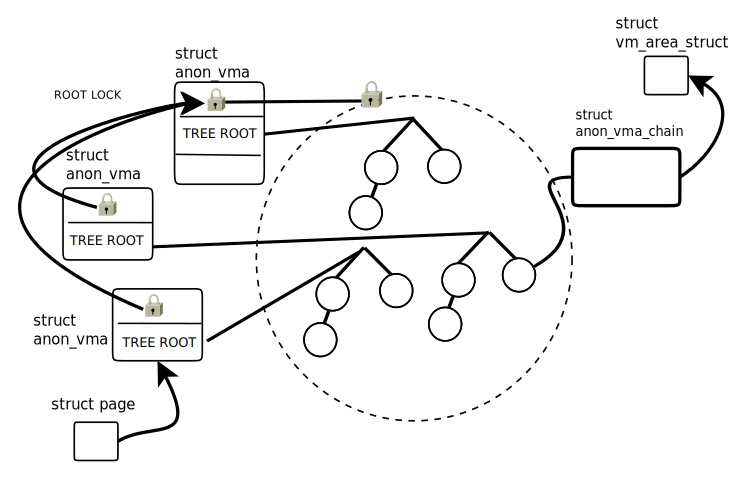
\includegraphics[scale=0.5]{fig/anon_vma_default}
\end{frame}


\begin{frame}{anonymous reverse mapping}
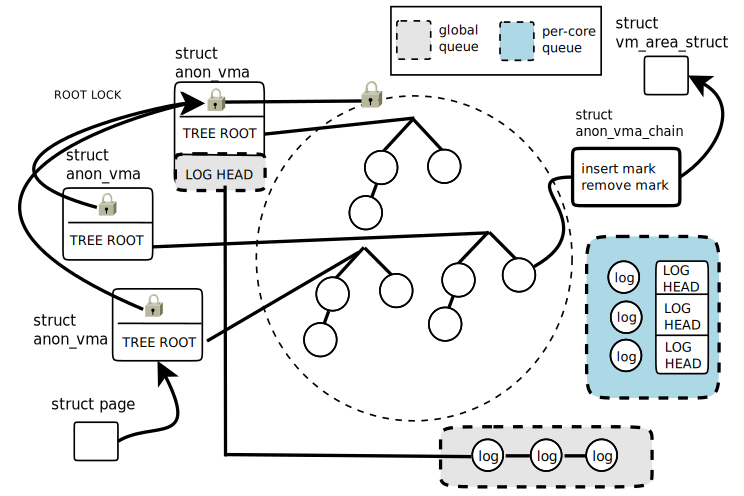
\includegraphics[scale=0.5]{fig/anon_vma}
\end{frame}


\begin{frame}{file mapping}
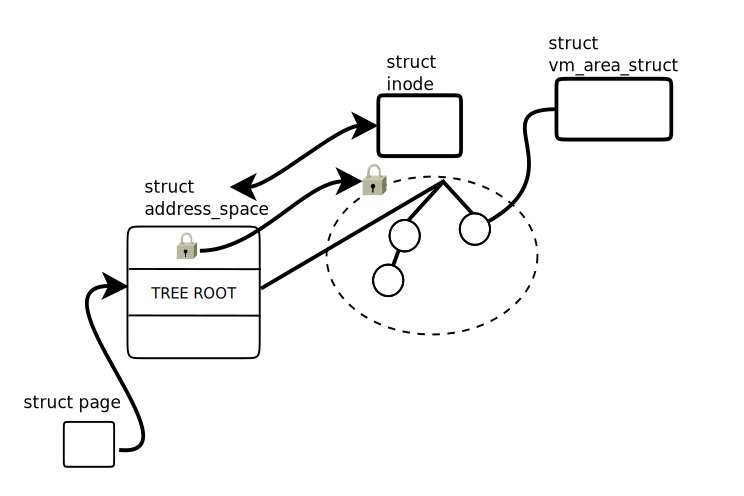
\includegraphics[scale=0.5]{fig/file_rmap_default}
\end{frame}


\begin{frame}{file mapping}
\includegraphics[scale=0.5]{fig/file_rmap}
\end{frame}



\begin{frame}{Evaluation}
    \begin{itemize}[<+-| alert@+>]
    \item We used four different experiment settings.
    \item 1. stock Linux
    \item 2. LDU + global queue
    \item 3. LDU + per-core queue
    \item 4. Harris linked list
    \end{itemize}
\end{frame}


\begin{frame}{Non-blocking algorithm - Harris linked list}
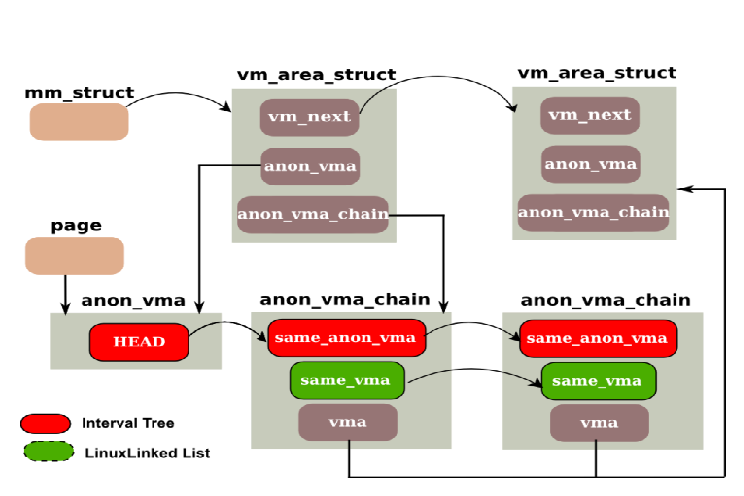
\includegraphics[scale=0.5]{fig/lockfree}
\end{frame}

\begin{frame}{Hardware specification}
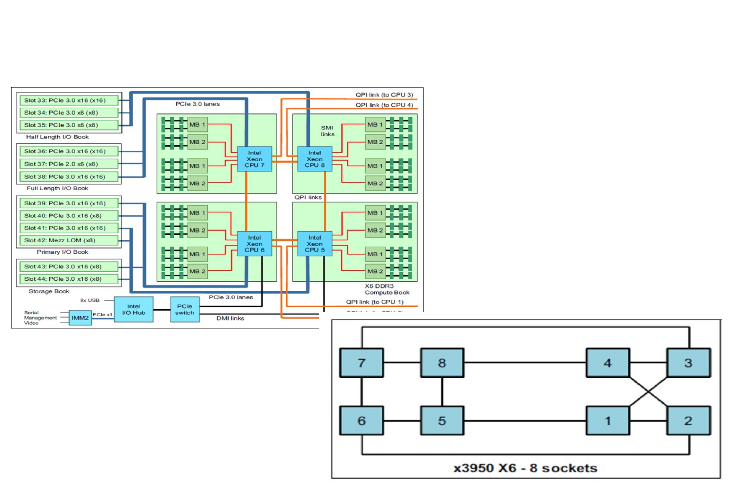
\includegraphics[scale=0.5]{fig/hardware}
\end{frame}


\begin{frame}{AIM7}
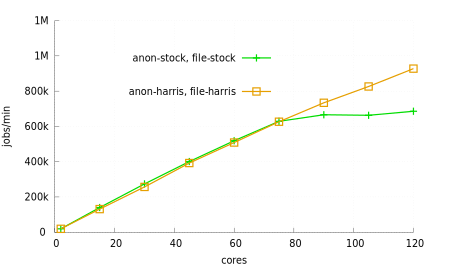
\includegraphics[scale=0.8]{graph/aim7}
\end{frame}

\begin{frame}{AIM7}
\includegraphics[scale=0.8]{graph/aim7_1}
\end{frame}

\begin{frame}{AIM7}
\includegraphics[scale=0.8]{graph/aim7_2}
\end{frame}


\begin{frame}{AIM7 - CPU utilization}
\includegraphics[scale=0.8]{graph/aim7_cpuutils}
\end{frame}

\begin{frame}{EXIM}
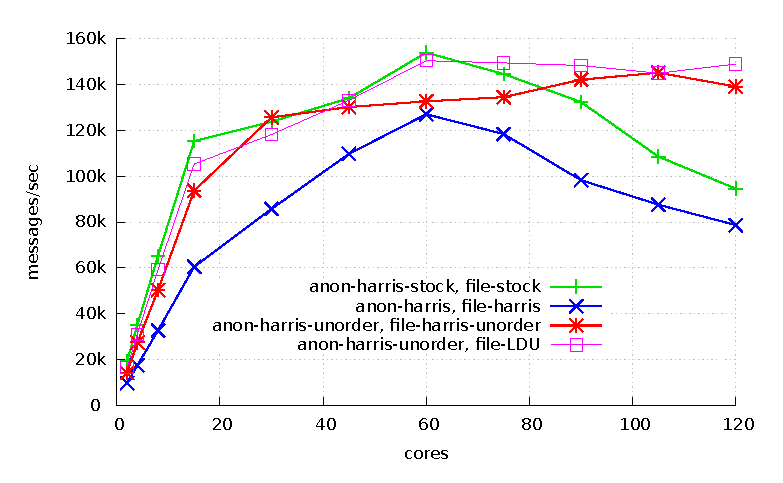
\includegraphics[scale=0.8]{graph/exim}
\end{frame}


\begin{frame}{EXIM - CPU utilization}
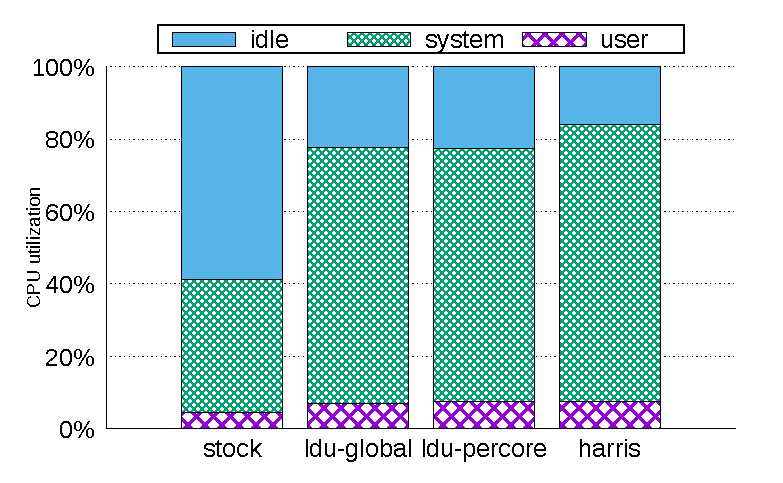
\includegraphics[scale=0.8]{graph/exim_cpuutils}
\end{frame}


\begin{frame}{Lmbench}
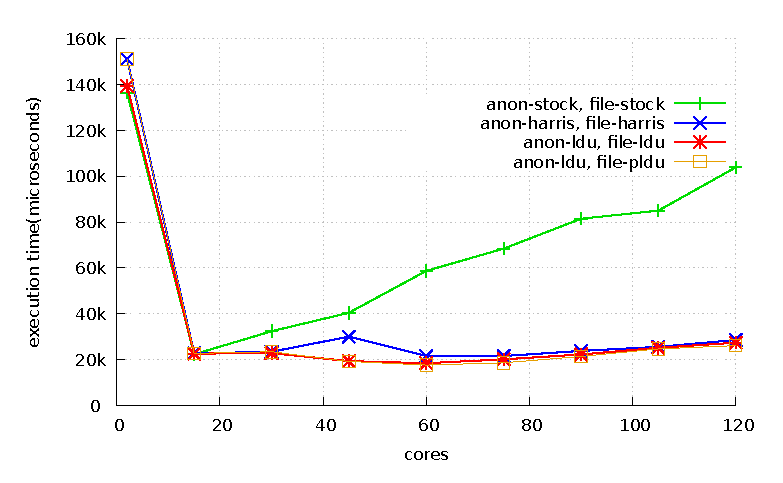
\includegraphics[scale=0.8]{graph/lmbench}
\end{frame}


\begin{frame}{Lmbench - CPU utilization}
\includegraphics[scale=0.8]{graph/lmbench_cpuutils}
\end{frame}


\begin{frame}{Update ratios}
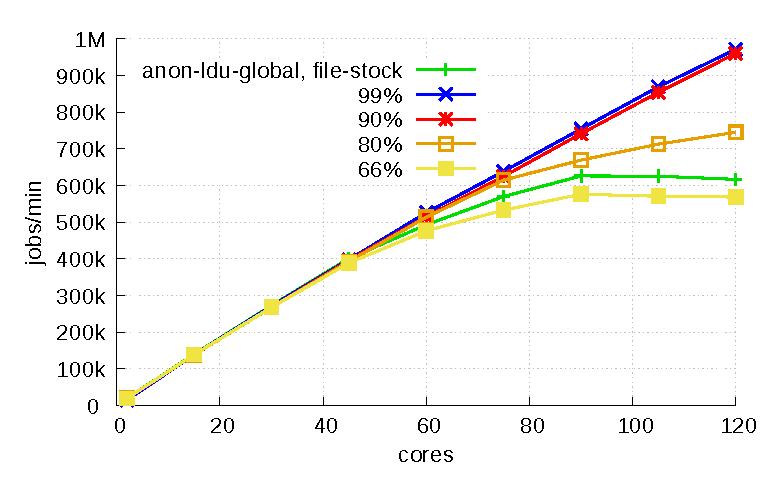
\includegraphics[scale=0.4]{graph/ratio_aim7_core}
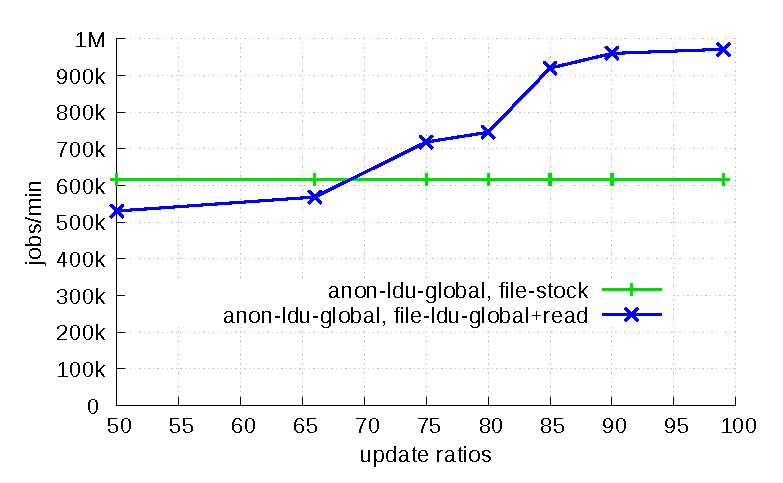
\includegraphics[scale=0.4]{graph/ratio_aim7}
\end{frame}

\begin{frame}{Related work}
\begin{itemize}
    \item Operating systems scalability.
    \begin{itemize}
    \item Create new operating systems.
    \item Optimize existing operating systems.
    \end{itemize}    
    \item Scalable lock.
    \begin{itemize}
    \item Queue-based locks.
    \item Hierarchical locks.
    \item Delegation techniques.
    \end{itemize}
    \item Scalable data structures.
    \begin{itemize}
    \item Different performances depending on their update ratios.
    \end{itemize}
    \end{itemize}
\end{frame}


\begin{frame}{Curriculum Vitae}
\includegraphics[scale=0.5]{cv/cv0}
\end{frame}

\begin{frame}{Curriculum Vitae}
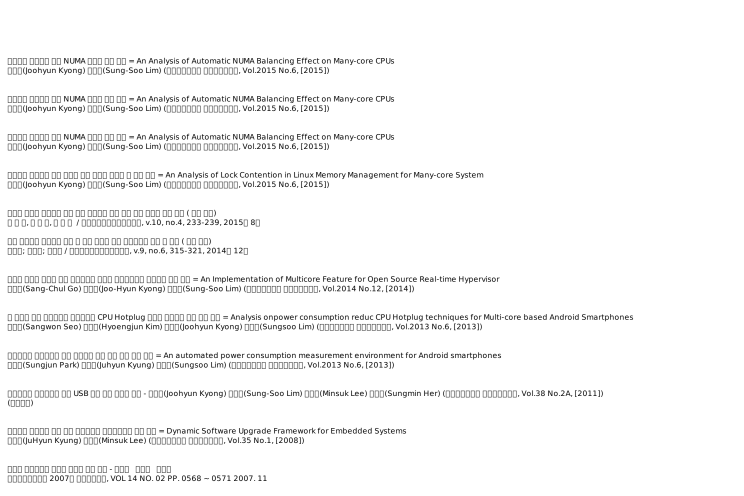
\includegraphics[scale=0.5]{cv/cv1}
\end{frame}

\begin{frame}{Curriculum Vitae}
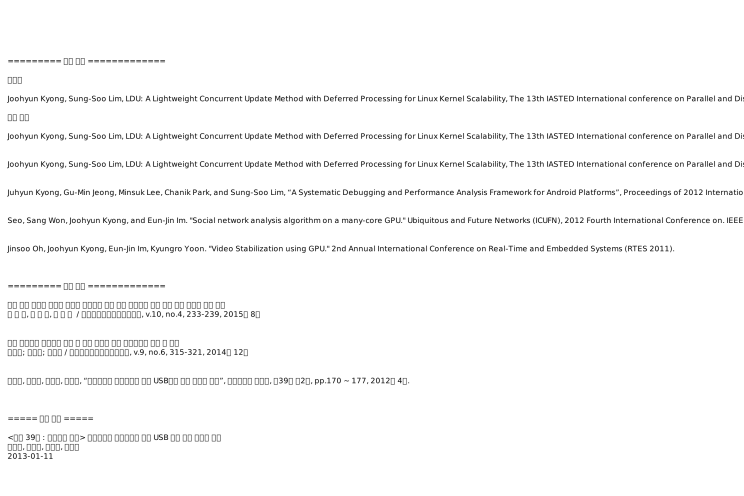
\includegraphics[scale=0.5]{cv/cv2}

\end{frame}
\begin{frame}{Conclusion}
	\begin{itemize}
	\item Background of research 
	\item LDU method and Evaluation
	\item Future plans and Summary
	\end{itemize}
\end{frame}


\begin{frame}{Conclusion}
    \begin{itemize}
    \item Background of research 
    \item LDU method and Evaluation
    \item Future plans and Summary
    \item \text{https://github.com/KMU-embedded/scalablelinux}
    \end{itemize}
\end{frame}


\end{document}
